\documentclass[quiz,addpoints,noanswers]{exam}

\usepackage[quiz]{../biology11}
\usepackage{chemformula}

\title{Quiz: Cell cycle (earned honors)}
\date{\today}
\author{\mobeardInstructorShort}

\begin{document}
\maketitle
%\begin{abstract}
%Today's quiz is a salute to Q1/Q2. This quiz should only take about \SI{5}{\minute}. Answers will be made available on Google Drive \SI{15}{\minute} after the quiz start time. 
%\end{abstract}

\begin{figure}[h]
\begin{center}
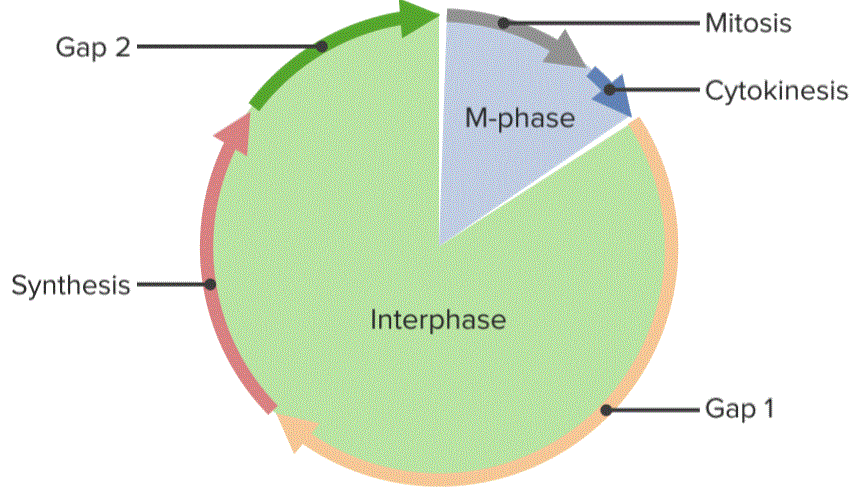
\includegraphics[width=3in]{cellcycle.png}
\end{center}
\caption{Cell cycle, divided into five phases. From \url{https://www.lecturio.com/magazine/the-cell-cycle/}}
\end{figure}

\begin{questions}
\question[1] What takes place during the portion labeled Gap 1 (G1) phase? 
\begin{solution}[1.25in]
\end{solution}

\question[1] What takes place during\footnote{Thanks to Charlie Guida '22 for spotting typo on the first version of this quiz.} the portion labeled Synthesis (S) phase?
\begin{solution}[1.25in]
\end{solution}

\question[1] What takes place during the portion labeled Gap 2 (G2) phase? 
\begin{solution}
\end{solution}

\clearpage
\question[1] What takes place during the portion labeled M phase? 
\begin{solution}[1.5in]
\end{solution}

\question[1]  What is a ``big'' question you are interested in about cell division (no wrong answers)? 
\begin{solution}[1in]
\end{solution}

\end{questions}
\end{document}